\chapter{Time Evolution}
Recall the expression for the superfluid state
\begin{equation}\label{eq:SF_psi}
\lvert \psi \rangle = C \sum_{j=0}^{\infty} \frac{\alpha^j}{\sqrt{j!}}\lvert j\rangle,
\end{equation}
Recent experimental advances have made it possible to change the Hamiltonian almost instantaneously, allowing for a wide array of new experiments. In the current section, we will look at the case of an SF Hamiltonian,
\begin{equation}\label{eq:SF_ham}
\hat{H} = -J \sum_{\braket{i,j}} \hat{a}_{i}^{\dag} \hat{a}_j,
\end{equation}
 present long enough for the condensate to reach the ground state in eq. \ref{eq:SF_psi} suddenly being switched to a pure Mott Hamiltonian,
\begin{equation}
 \hat{H} = \frac{U}{2} \sum_{i} \hat{n}_i \left( \hat{n}_i -1 \right).
\end{equation}
%
In this case, the time evolution of the state can be described by
\begin{equation}
\lvert \psi (t) \rangle = C \sum_{j=0}^{\infty} \e^{-it \frac{U}{2} j(j-1)}\frac{\alpha^j}{\sqrt{j!}}\lvert j\rangle,
\end{equation}
and since $j(j-1)/2\in \mathbb{N}$ for all $j$, we will regain the superfluid state at times $p2\pi/U$,
\begin{equation}
\lvert \psi (p2\pi/U) \rangle = \lvert \psi (0) \rangle,
\end{equation}
for all integers $p$, whereby we should see a revival of the condensate fraction, as described in \ref{CondFrac}.

\section{Numerical Results}
Further testing the applicability of the MPS formalism using ITensor library for time evolution, we evolved an SF state in time first with respect to a pure Mott Hamiltonian ($U=1$, $J=0$), then with respect to a slightly different Hamiltonian ($U=2$, $J=0.03$).

\subsection{$U=1$, $J=0$}
Mott time evolution on a superfluid state was performed for various unit occupancy systems with complex time steps $t_{1,2}=\frac{1\pm i}{2}t$ as described in \cite{cmplx_t}, and the condensate fraction was subsequently plotted as a function of time. The initial SF state was found by DMRG with the Hamiltonian in eq. \ref{eq:SF_ham}.
\begin{figure}[h!]
    \centering
    \begin{subfigure}[t]{0.49\textwidth}
        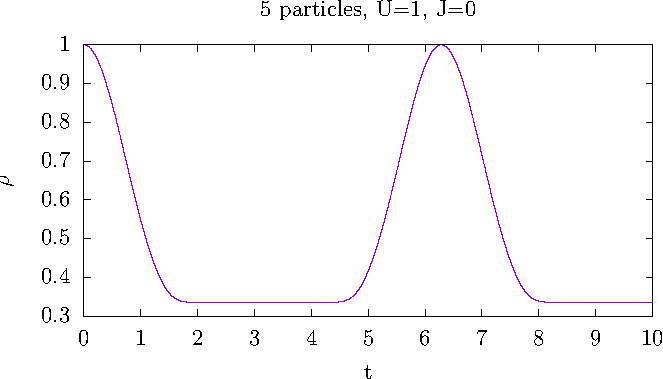
\includegraphics[width=\textwidth]{Figures/TimeEvo5_U1_J0.pdf}
        \caption{\textit{Condensate fraction calculated from a 5 particle, 5 site MPS after performing 10 DMRG sweeps with an SF Hamiltonian ($J=1$, $U=0$) followed by time evolution with a Mott Hamiltonian ($J=0, U=1$).}}
        \label{fig:TimeEvo5_U1_J0}
    \end{subfigure}
    ~
    \begin{subfigure}[t]{0.49\textwidth}
        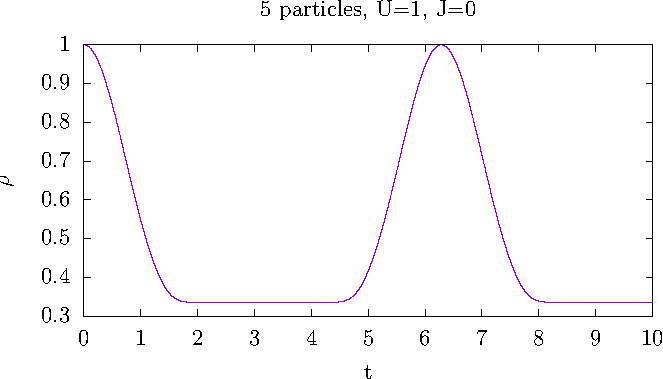
\includegraphics[width=\textwidth]{Figures/TimeEvo50_U1_J0.pdf}
        \caption{\textit{Condensate fraction calculated from a 50 particle, 50 site MPS after performing 20 DMRG sweeps with an SF Hamiltonian ($J=1$, $U=0$) followed by time evolution with a Mott Hamiltonian ($J=0, U=1$).}}
        \label{fig:TimeEvo50_U1_J0}
    \end{subfigure}    
\end{figure}
Figure \ref{fig:TimeEvo5_U1_J0} shows time evolution for 5 particles, whereas \ref{fig:TimeEvo50_U1_J0} is for 50 particles \\(note: figure not yet made)\\ with $U=1$, the period, that is, the time for a full revival of the condensation fraction to occur, can be seen from both figures to be $T=2\pi$. 

WAITING FOR DATA...

\subsection{$U=2$, $J=0.03$}
Performing time evolution on an SF state with a nonzero $J$, the condensate fraction does not achieve full revival, but instead the phases of the individual particle states interfere with each other more and more for each cycle, leading to a decreasing maximal condensate fraction and some spurious lumps in between the peaks, see fig. \ref{fig:TimeEvo5_U2_J0_03}. The period of revival is $T=\pi$, since now $U=2$.

\begin{figure}[h!]
    \centering
    \begin{subfigure}[t]{0.49\textwidth}
        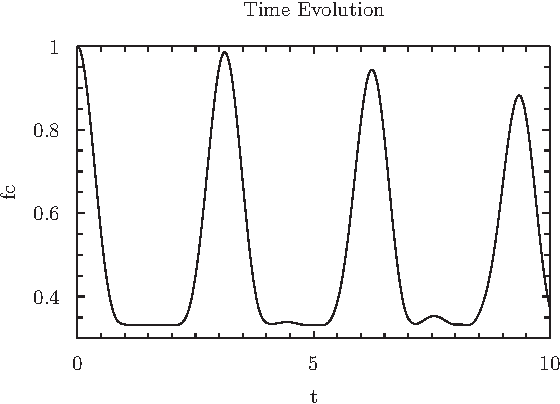
\includegraphics[width=\textwidth]{Figures/TimeEvo5_U2_J0_03.pdf}
        \caption{\textit{Condensate fraction calculated from a 5 particle, 5 site MPS after performing 10 DMRG sweeps with an SF Hamiltonian ($J=1$, $U=0$) followed by time evolution with a ($J=0.03, U=2$) Hamiltonian.}}
        \label{fig:TimeEvo5_U2_J0_03}
    \end{subfigure}
    ~
    \begin{subfigure}[t]{0.49\textwidth}
        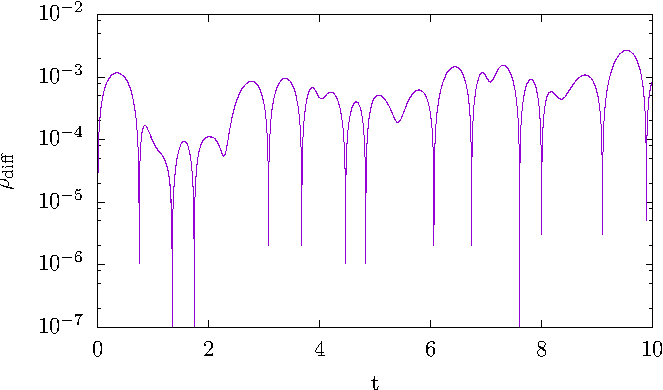
\includegraphics[width=\textwidth]{Figures/TimeEvo5_U2_J0_03_VS_ExactDiag.pdf}
        \caption{\textit{Condensate fraction calculated from a 5 particle, 5 site MPS after performing 10 DMRG sweeps with an SF Hamiltonian ($J=1$, $U=0$) followed by time evolution with a ($J=0.03, U=2$) Hamiltonian compared with the same calculations done with exact diagonalization.}}
        \label{fig:ExDiagComp_U2_J0_03}
    \end{subfigure}
\end{figure}

In fig. \ref{fig:ExDiagComp_U2_J0_03}, the absolute difference between the condensate fraction calculated by MPS formalism and that calculated by exact diagonalization is plotted. The disagreement, while still small at $t=10$, is expected to grow larger for larger times, as the MPS does a series of truncations each time the time evolution MPO is applied to avoid increasing the bond dimension of the MPS, whereas exact diagonalization using the Lanczos algorithm detailed in [Lanczos, C. "An iteration method for the solution of the eigenvalue problem of linear differential and integral operators", J. Res. Nat’l Bur. Std. 45, 255-282 (1950)] is limited mainly by machine precision.